%-*- mode: LaTeX; -*-

%Will show the results. Discussion in ch. 7. 
%Table of grown undoped samples
	%(Substrate face) Only carbon?
	%Growth temperature and time (one or two step process)
	%Thickness
	%Terrace coverage fraction
%Figure example to show where coverage is (edges)

%Table with all doped samples
	%Growth T and t
	%Thickness
	%Source doping
	%Color
	%Growth mode (indirect or direct)
	
%Absorption plots
	%Different doping and one undoped
	%Show that both direct and indirect grown samples show B-peaks
	%(Change axes to find band gap) Do I really need this, what conclusions?
	
	%Show that E18 and E19 samples give proper abs
		%Note that none of the samples give third transition
	%Show that Indirect too gives abs, show BGe18 

%LTPL
	%Show seed spectrum and compute the N-concentration
	%Show some of the B-doped. No radiation
	%Show new data with 4H-radiation B-N. 
	
%RTPL
	%...
	

\chapter{Results}
\label{sec:results}
In this chapter, the results of the experiments are shown. The chapter is divided into two parts. The first part shows the results for unintentionally doped seed growth, whereas the second part shows the results of B-doped samples. The results are further discussed in chapter \ref{sec:discussion}. 

\section{On seed growth}
\label{sec:results:seeds}
This section contains the results of characterization of unintentionally doped 3C-SiC seeds. To investigate growth of seeds to be used for B-doping, seeds were grown on both carbon and silicon face of the 4H-SiC. Table \ref{tab:seeds} shows the growth conditions and properties of the seeds grown on carbon face. The sample thickness is excluding the substrate thickness. Terrace coverage indicates the percentage of the sample terrace (or facet) covered by 3C-SiC rather than any other polytype. Not all sample coverages were measured quantitively, but the percentages in the table are thought to be representative. The silicon face seeds were all grown with a two step temperature ramp up sheme, with temperatures 1850/1925 $^\circ$C during times of 0:30/1:00 (hours/minutes). Nine out of ten of the silicon face grown seeds had a terrace coverage of 100 \%, whereas none of the carbon face samples had complete terrace coverage. The terrace coverage was estimated from optical micrographs.

\begin{table}[h]
\caption{Growth conditions of seeds of undoped 3C-SiC grown on the carbon face of the substrate. For samples grown using a two stage temperature ramp up, the temperatures and growth times for each step are both shown.}
\label{tab:seeds}
\begin{center}
\begin{tabular}{l c c c c}
  \hline                       
  \hline       
  \vspace{1mm}
   & \small{Temperature [$^\circ$C]} & \small{Time [h:min]} & \small{Sample thickness [$\mu$m]} & \small{Terrace coverage [\%]}\\
    \hline
  S1 & 1825 & 4:00 & 700 & 40\\
  S2 & 1850/1925 & 0:30/1:00 & 800 & 20\\
  S3 & 1850/1925 & 0:30/1:00 & 800 & \\
  S4 & 1850/1925 & 0:30/1:00 & 900 & 30\\
  S5 & 1875/1925 & 0:15/1:00 & 800 & 50\\
  S6 & 1925 & 1:00 & 700 & 20\\
  S7 & 1925 & 1:00 & 700 & \\
  \hline  
\end{tabular}
\end{center}
\end{table}


Figures \ref{fig:carbon_seed1} and \ref{fig:carbon_seed2} show representative micrographs of the terrace of carbon face grown seed S5. Figure \ref{fig:carbon_seed1} shows a reflection mode micrograph. It can clearly be seen that there are a few large areas of different polytypes. The hexagonal polytype regions show spiral growth, which on carbon face 4H-SiC manifests as a star shape. The 3C-SiC regions look smoother, and show some of the characteristic triangle shapes. Figure \ref{fig:carbon_seed2} shows a Nomarski mode micrograph, showing clear contrast between the different polytype regions. 

\begin{figure}[h]
\centering
\begin{minipage}{.5\textwidth}
  \centering
  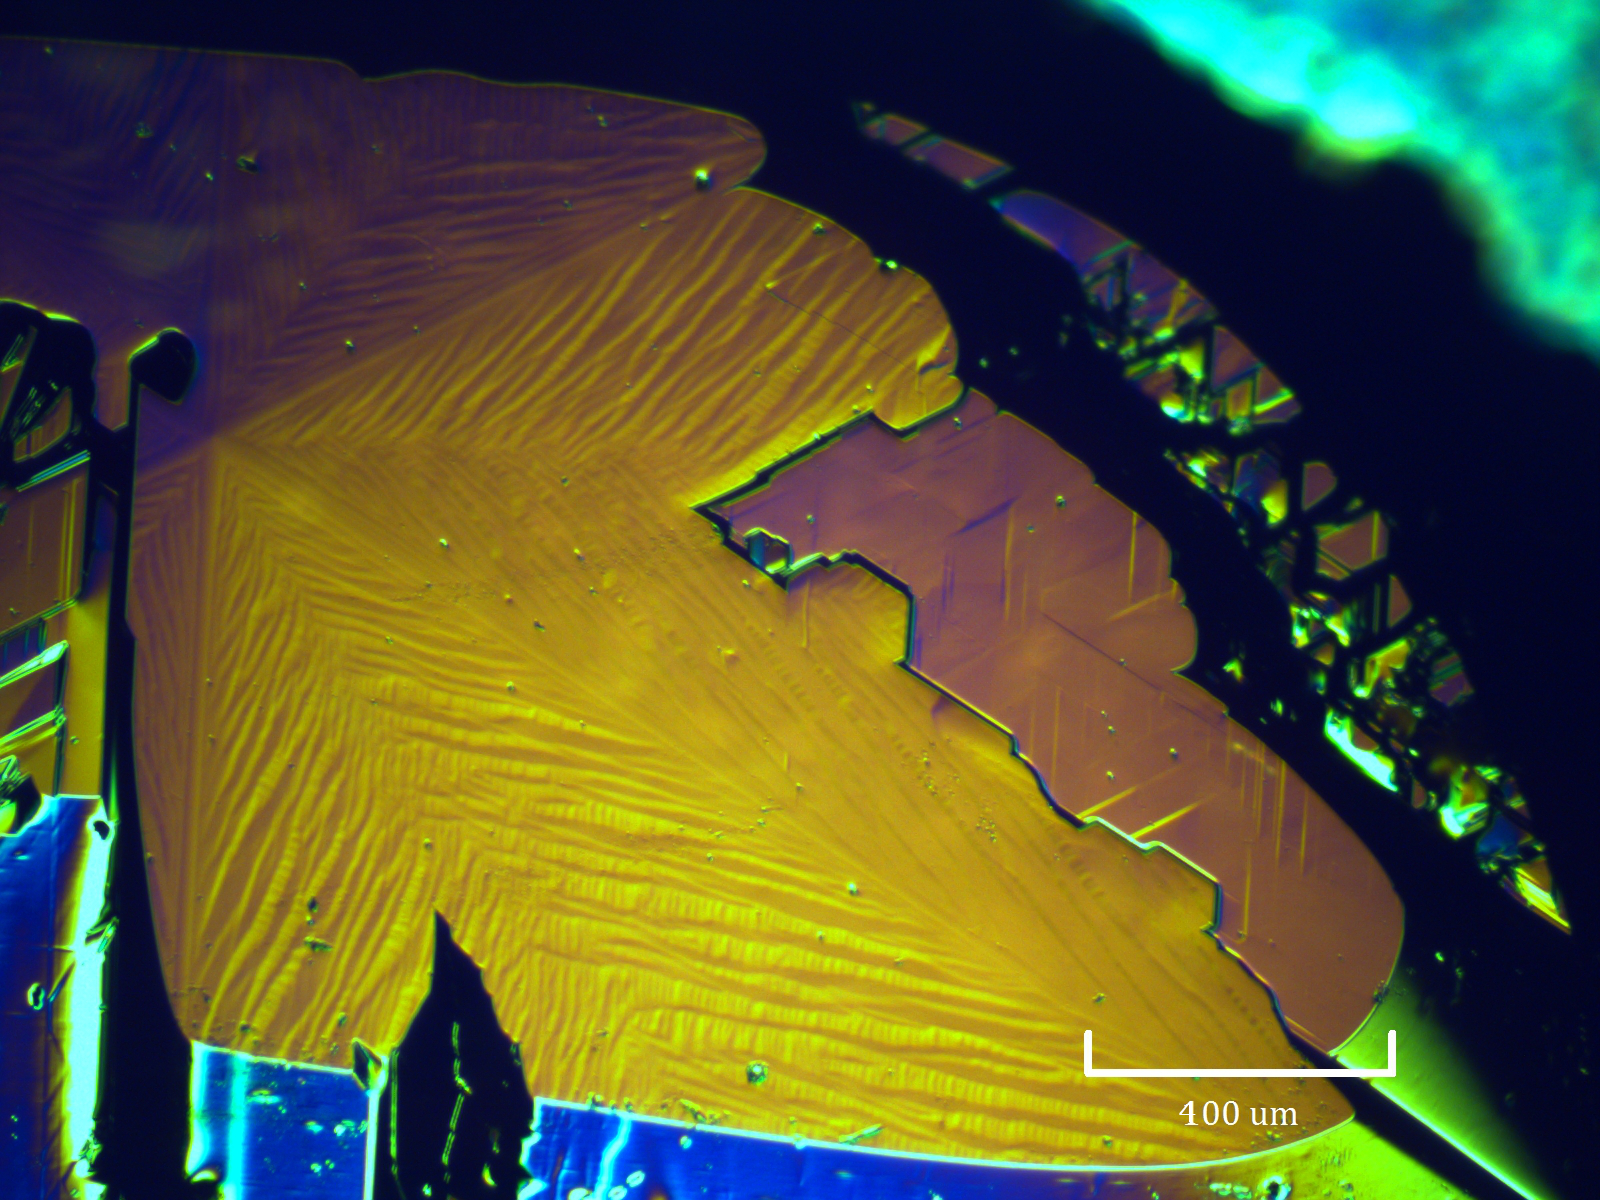
\includegraphics[scale=0.1]{C_seed1.jpg}
  \captionof{figure}{Reflection mode micrograph of the facet of C-face seed S5.}
  \label{fig:carbon_seed1}
\end{minipage}%
\begin{minipage}{.5\textwidth}
  \centering
  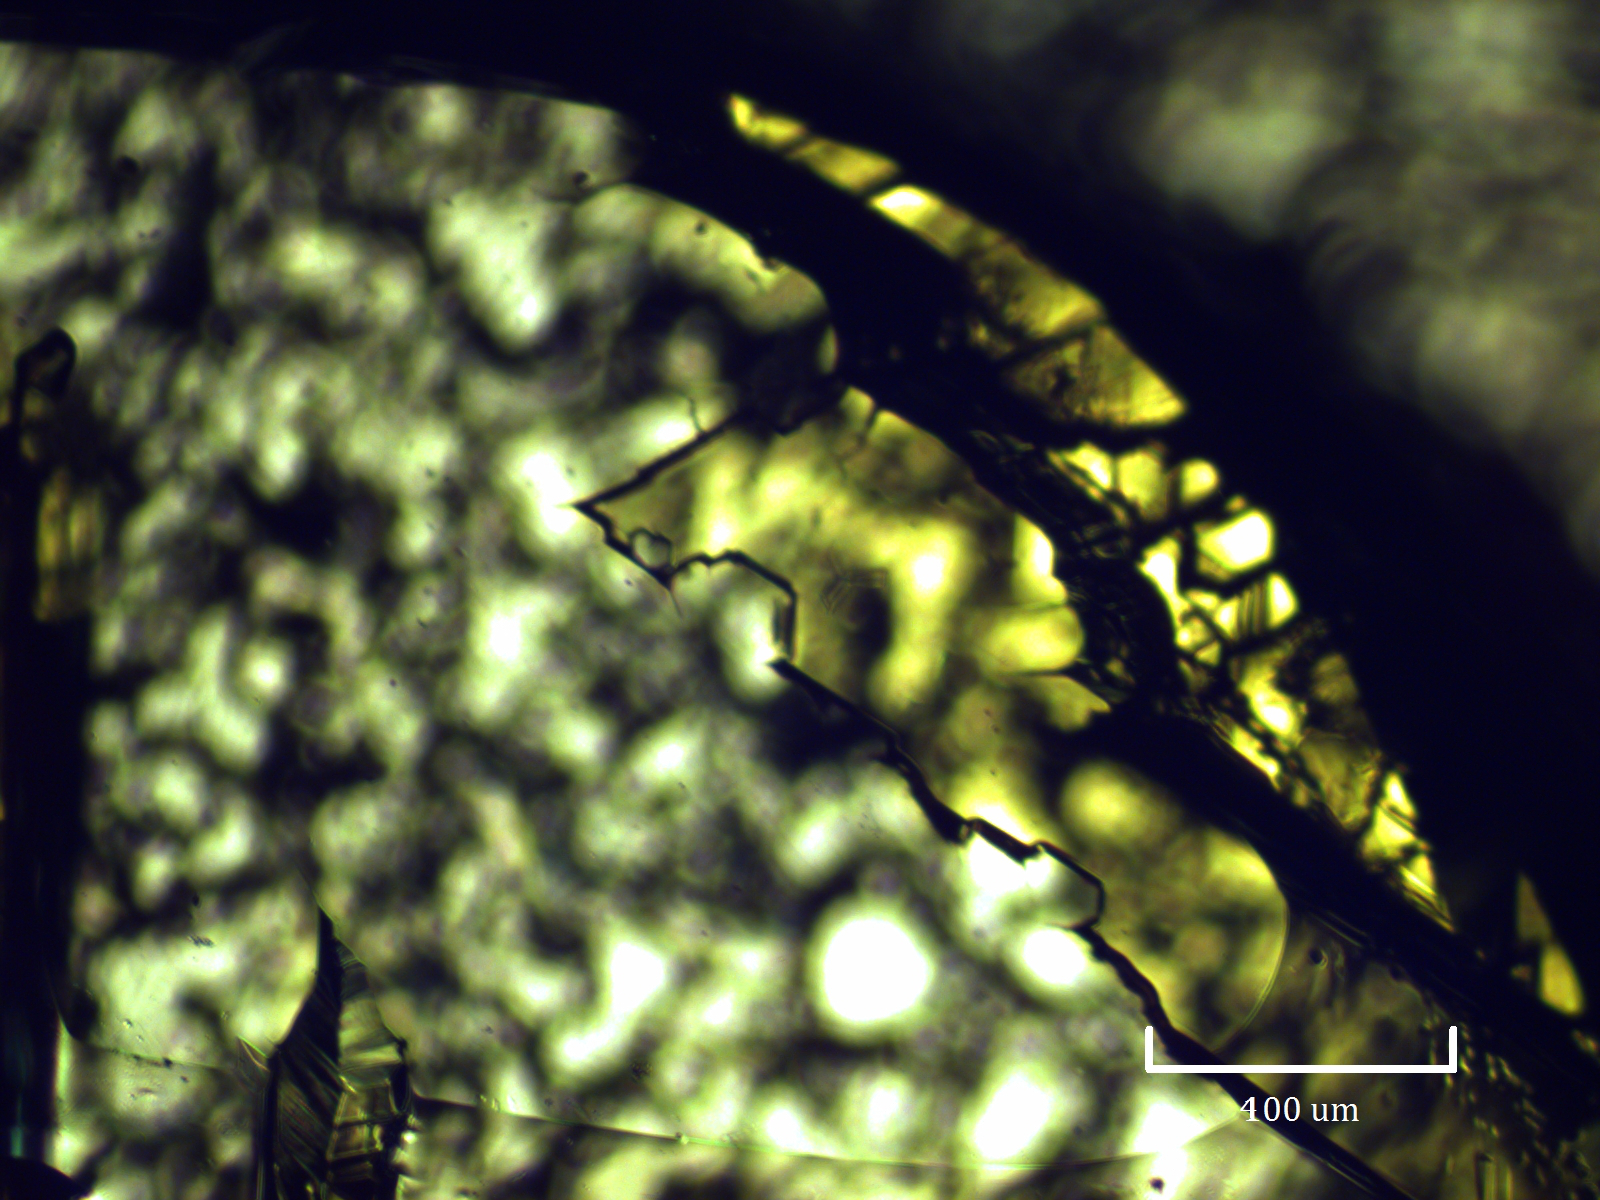
\includegraphics[scale=0.1]{C_seed2.jpg}
  \captionof{figure}{Nomarski transmission mode micrograph of the facet of C-face seed S5.}
  \label{fig:carbon_seed2}
\end{minipage}
\end{figure}

Figure \ref{fig:silicon_seed} shows a reflection mode micrograph of a silicon face grown seed. On this sample the whole terrace is covered with the 3C-SiC polytype. This micrograph is representative of the Si-face grown seeds, most of which had complete terrace coverage. 

\begin{figure}[H]
\begin{center}
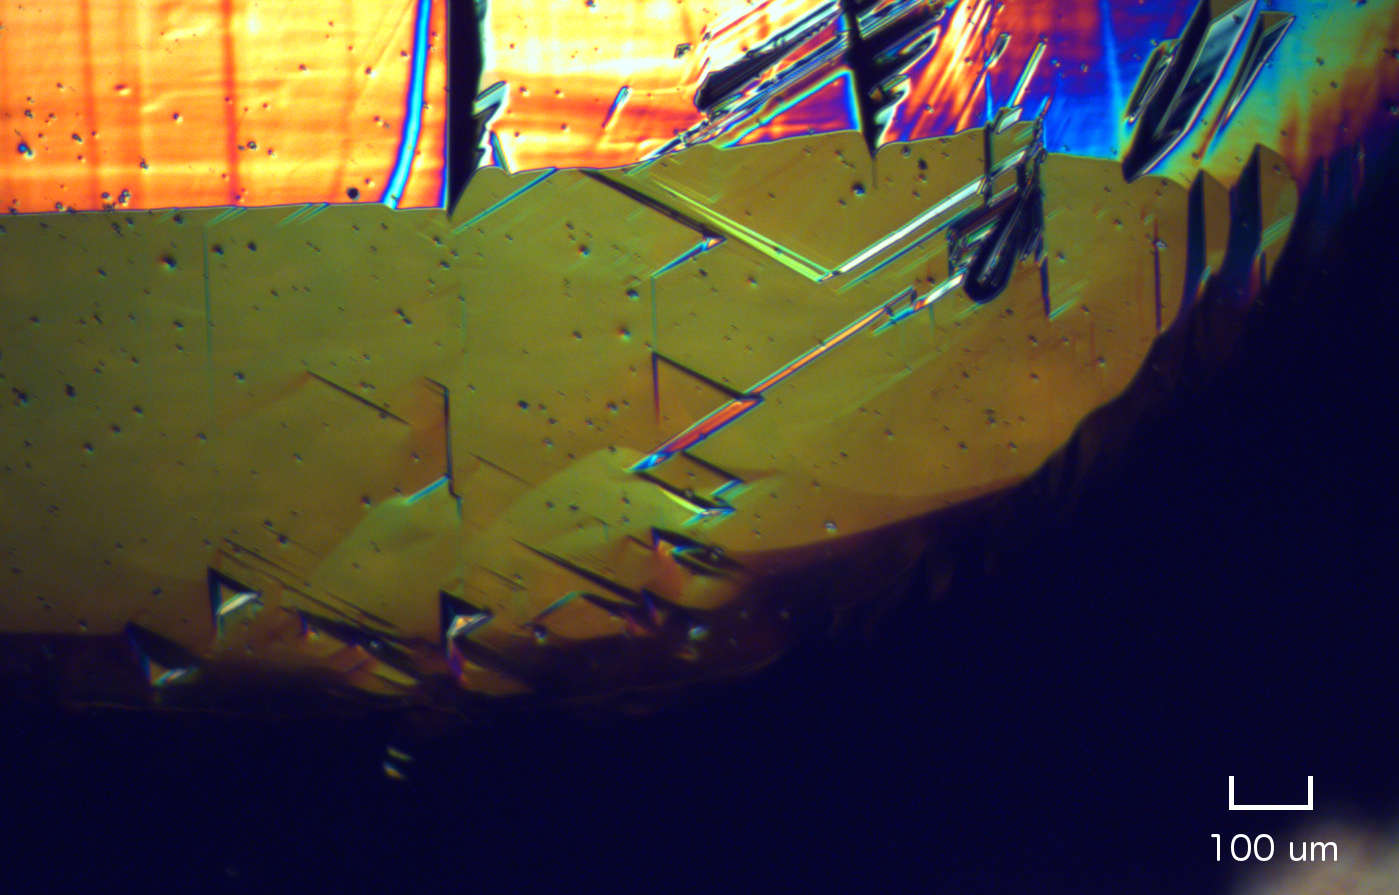
\includegraphics[scale=0.15]{undoped_Si_face.jpg}
\caption{Reflection mode micrograph of the facet of a Si-face seed.
\label{fig:silicon_seed}}
\end{center}
\end{figure}




\section{On B-doped samples}
\label{sec:results:doped}
This section shows the results of characterization of B-doped samples. Table \ref{tab:doped_samples} shows the growth conditions and sample thicknesses of the grown B-doped samples. The thickness is measured for the doped layer, excluding both the substrate and the undoped seed. The growth mode is the stacking order of the doped and undoped source materials in the crucible, as described in section \ref{sec:growth:fsgp:doping}. The \emph{Seed} column displays whether the sample was grown on a 3C-SiC seed or directly on a 4H-SiC 4$^\circ$ off-axis substrate. All substrates used for B-doped samples are Si-face, and the seeds except for D6 are grown on Si-face. 

\begin{table}[h]
\caption{Growth conditions of the doped samples are shown in this table. The growth mode describes which samples are grown using direct or indirect doping methods. These methods are described in section \ref{sec:growth:fsgp:doping}. The doping concentration is given for the source material. The seed column indicates whether the B-doped sample is grown on a 3C-SiC seed or on a 4H-SiC substrate.} 
\label{tab:doped_samples}
\begin{center}
\begin{tabular}{l c c c c c r}
  \hline                       
  \hline       
  \vspace{1mm}
   & \small{Temp. [$^\circ$C]} & \small{Time [h:min]} & \small{Thickness [$\mu$m]} & \small{Doping [cm$^{-3}$]} & Mode & Seed\\
    \hline
  D1 &  &  &  & 10$^{18}$&Direct & Yes\\ %S1
  D2 & 1825 & 2:30 & 350 & 10$^{18}$&Direct & Yes\\ %S3
  D3 & 1825 & 3:00 & 360 & 10$^{18}$&Direct & Yes\\	%S2
  D4 &  &  & 440 & 10$^{19}$&Direct & Yes\\ %S1
  D5 & 1825 & 2:30 & 320 & 10$^{19}$&Direct & Yes\\ %S2
  D6 &  &  &  & 10$^{20}$&Direct & Yes\\%S1
  D7 & 1825 & 2:30 & 220 & 10$^{20}$&Direct & Yes\\%S2
  D8 & 1825 & 2:30 & 380 & 10$^{18}$&Indirect & Yes\\%S3
%  2 & XXX & X:XX & X & 10$^{20}$&Indirect\\%S2 %BG proper
  D9 & 1825 & 2:30 & 380 & 10$^{20}$&Indirect & No\\%S3
  
  \hline  
\end{tabular}
\end{center}
\end{table}


\begin{figure}[h]
\begin{center}
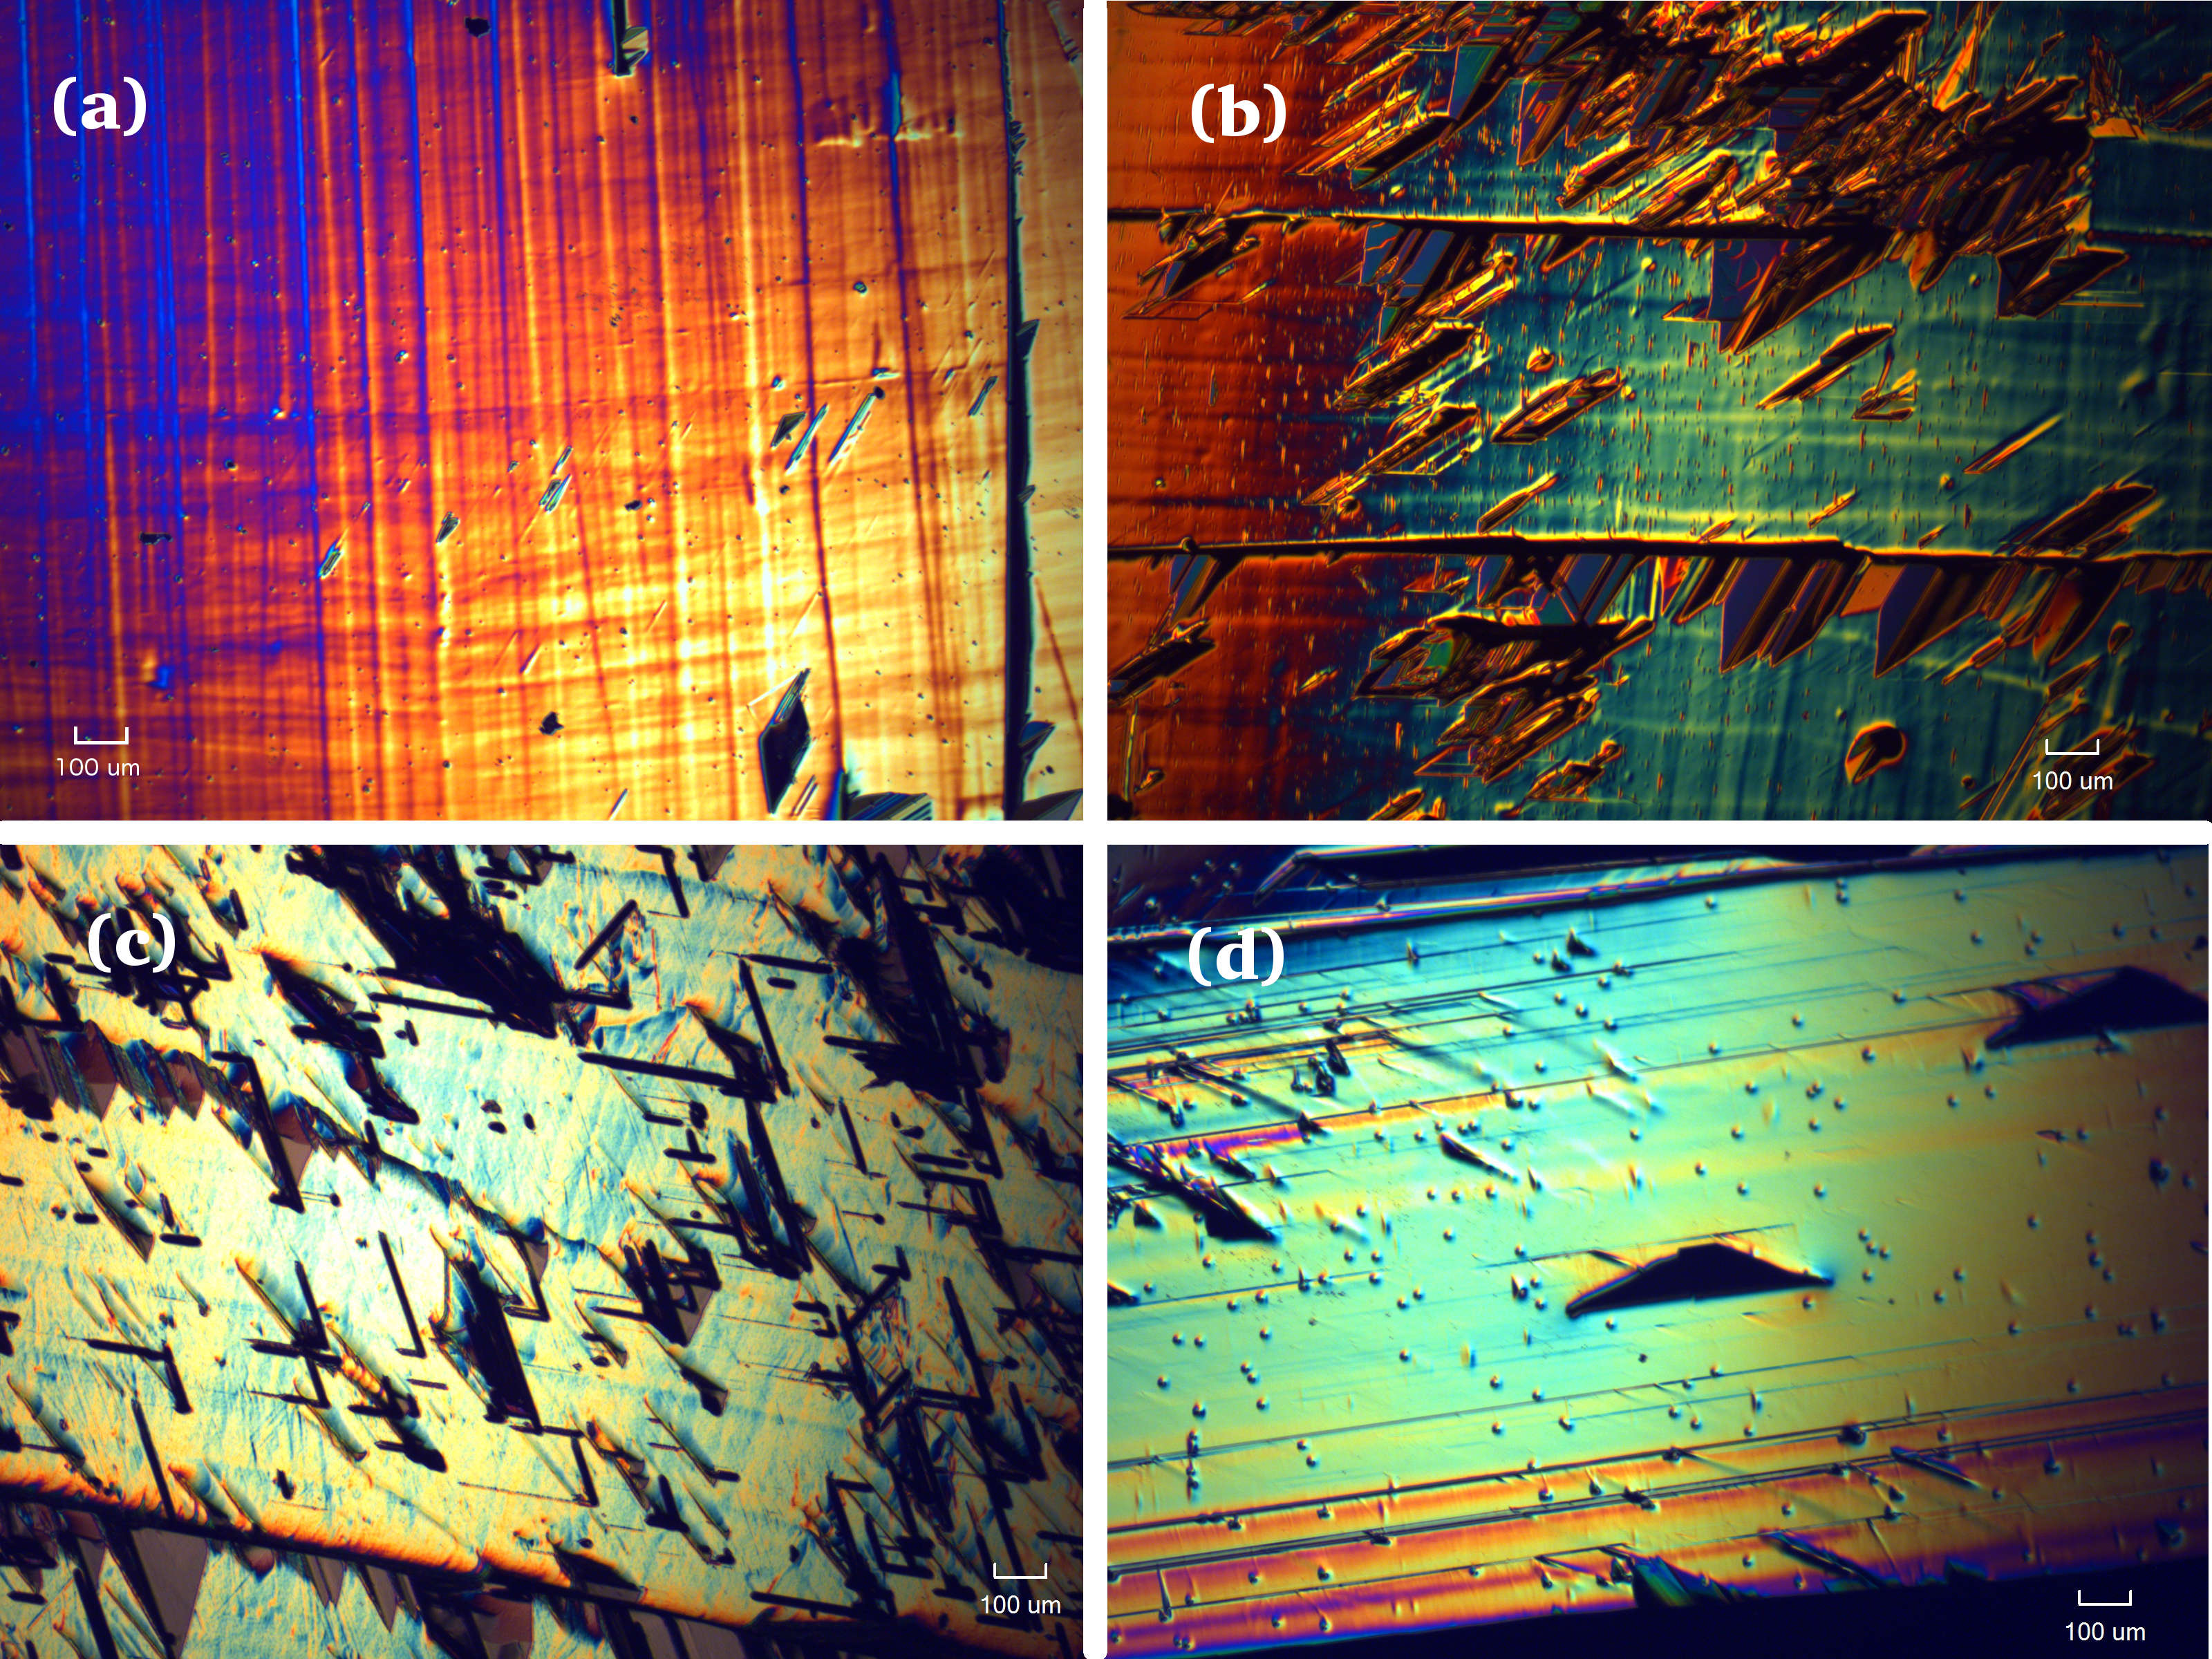
\includegraphics[scale=0.10]{doped_series_four.jpg}
\caption{Micrographs of an undoped sample (a), doped sample number D1 (b), doped sample number D4 (c) and doped sample number D6 (d).
\label{fig:B_doped_micrographs1}}
\end{center}
\end{figure}

Figure \ref{fig:B_doped_micrographs1} shows the surface morphology of an undoped sample (a), doped sample number D1 (b), doped sample number D4 (c) and doped sample number D6 (d). It is clearly seen that the undoped sample has a better surface quality compared to (b) and (c), but (d) which is grown with a highly doped source shows good surface quality. Sample D7, grown under similar conditions as D6, shows a much worse surface, comparable with that in (c). The micrographs are representative for the whole surface morphology of the samples. It should be noted that the samples (b)-(d)   are grown using a source material doped with dopant concentration of 10$^{18}$, 10$^{19}$ and 10$^{20}$ cm$^{-3}$ respectively.

Figure \ref{fig:B_doped_micrographs2} shows micrographs of samples D1 (a) and D8 (b). It should be noted that the two samples are grown with direct and indirect doping methods respectively. It can be seen that the sample surface quality is similar in the two samples. 

\begin{figure}[h]
\begin{center}
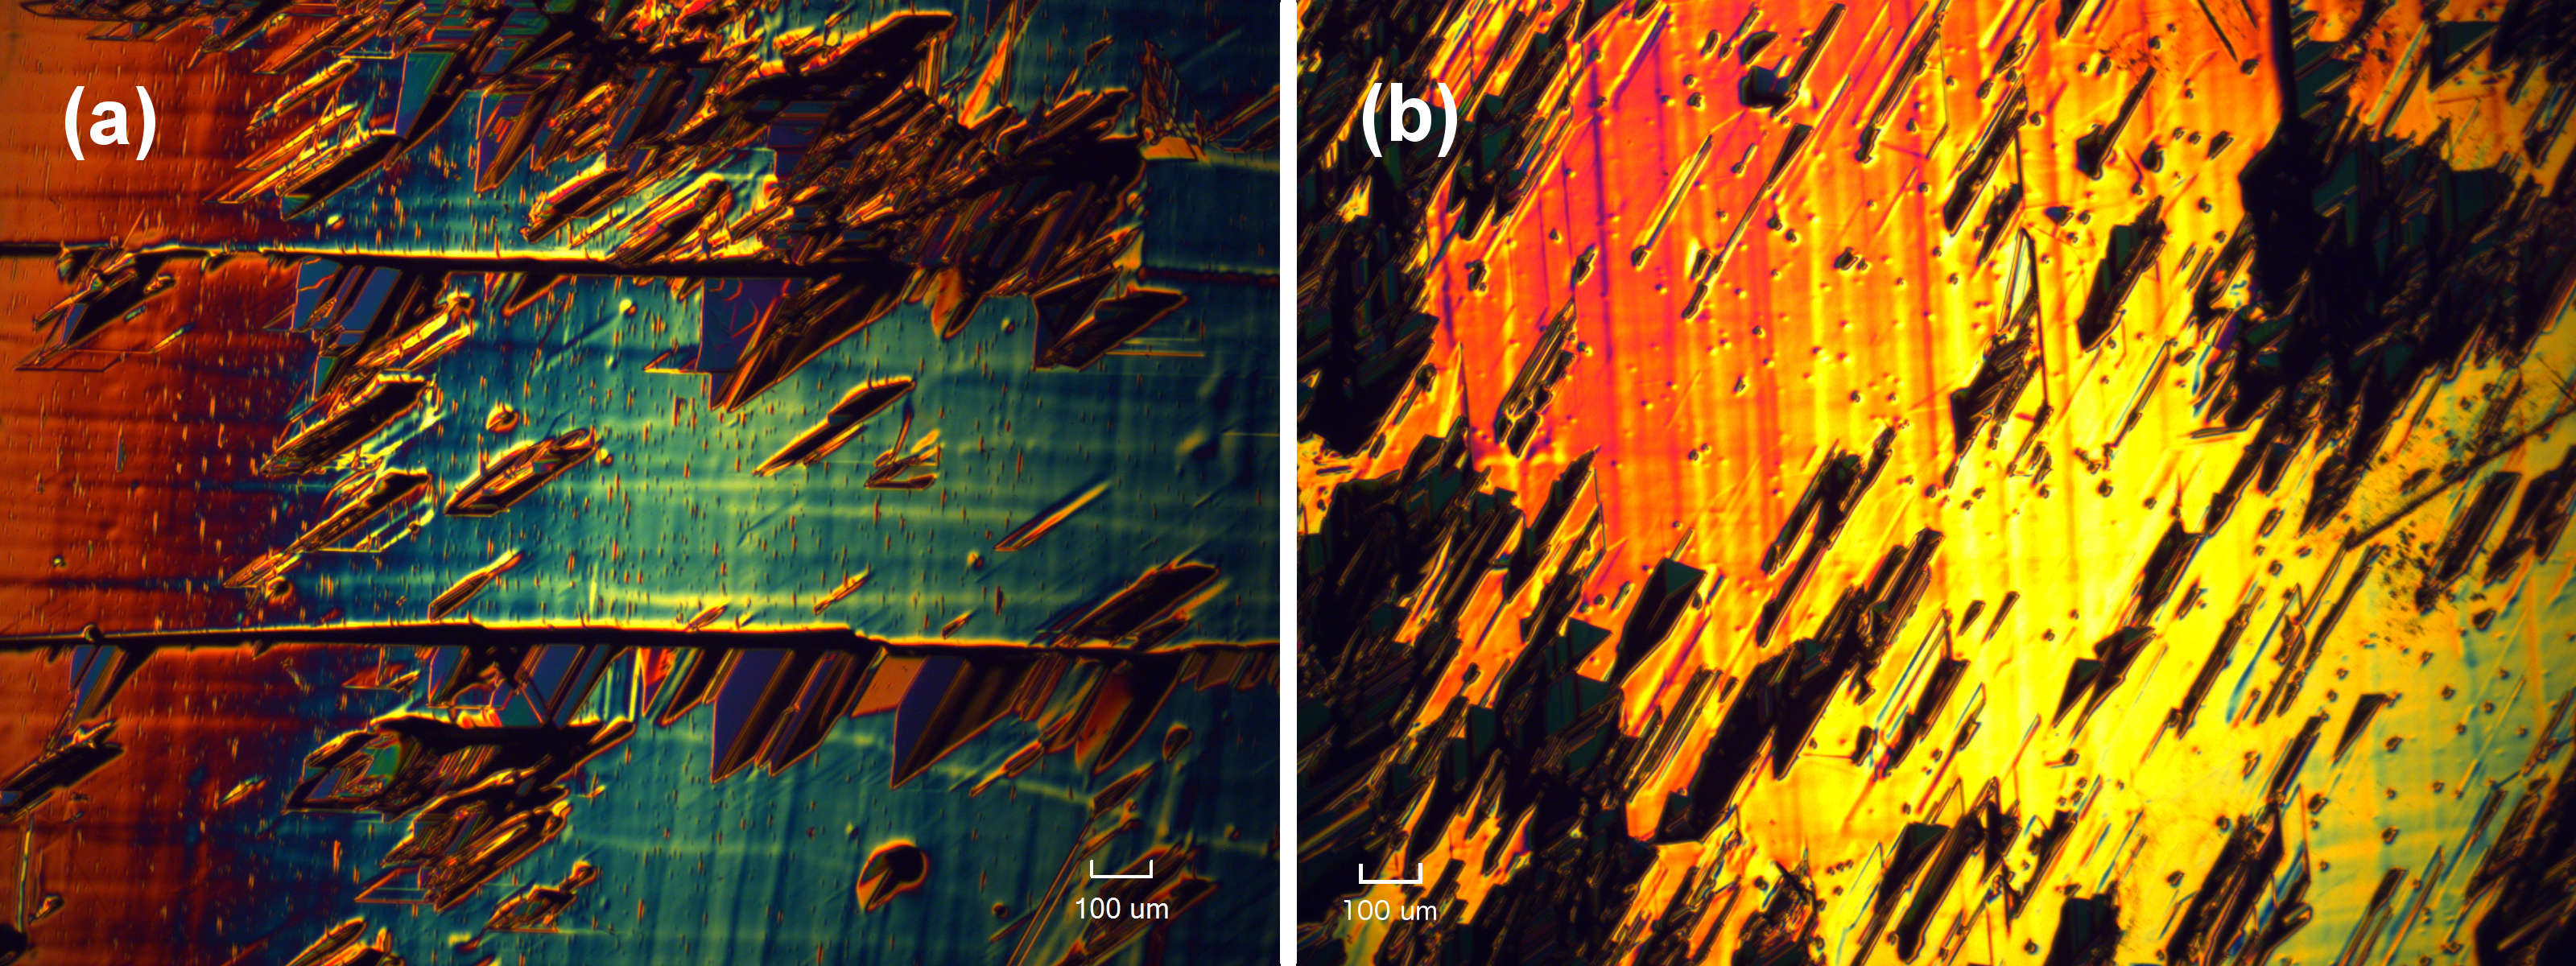
\includegraphics[scale=0.11]{direct_indirect_e18.jpg}
\caption{Micrographs of samples D1 (a) and D8 (b). 
\label{fig:B_doped_micrographs2}}
\end{center}
\end{figure}


Figure \ref{fig:BGe20_micrograph} shows reflection mode micrographs of samples D6 (a) and D9 (b). These samples are grown with direct and indirect growth methods respectively. Both samples show comparable surface morphology. In (c) a transmission mode micrograph of D9 is shown. It can be seen that there are two different polytypes in the sample. The brighter area in the center is a foreign polytype inclusion. 

\begin{figure}[h]
\begin{center}
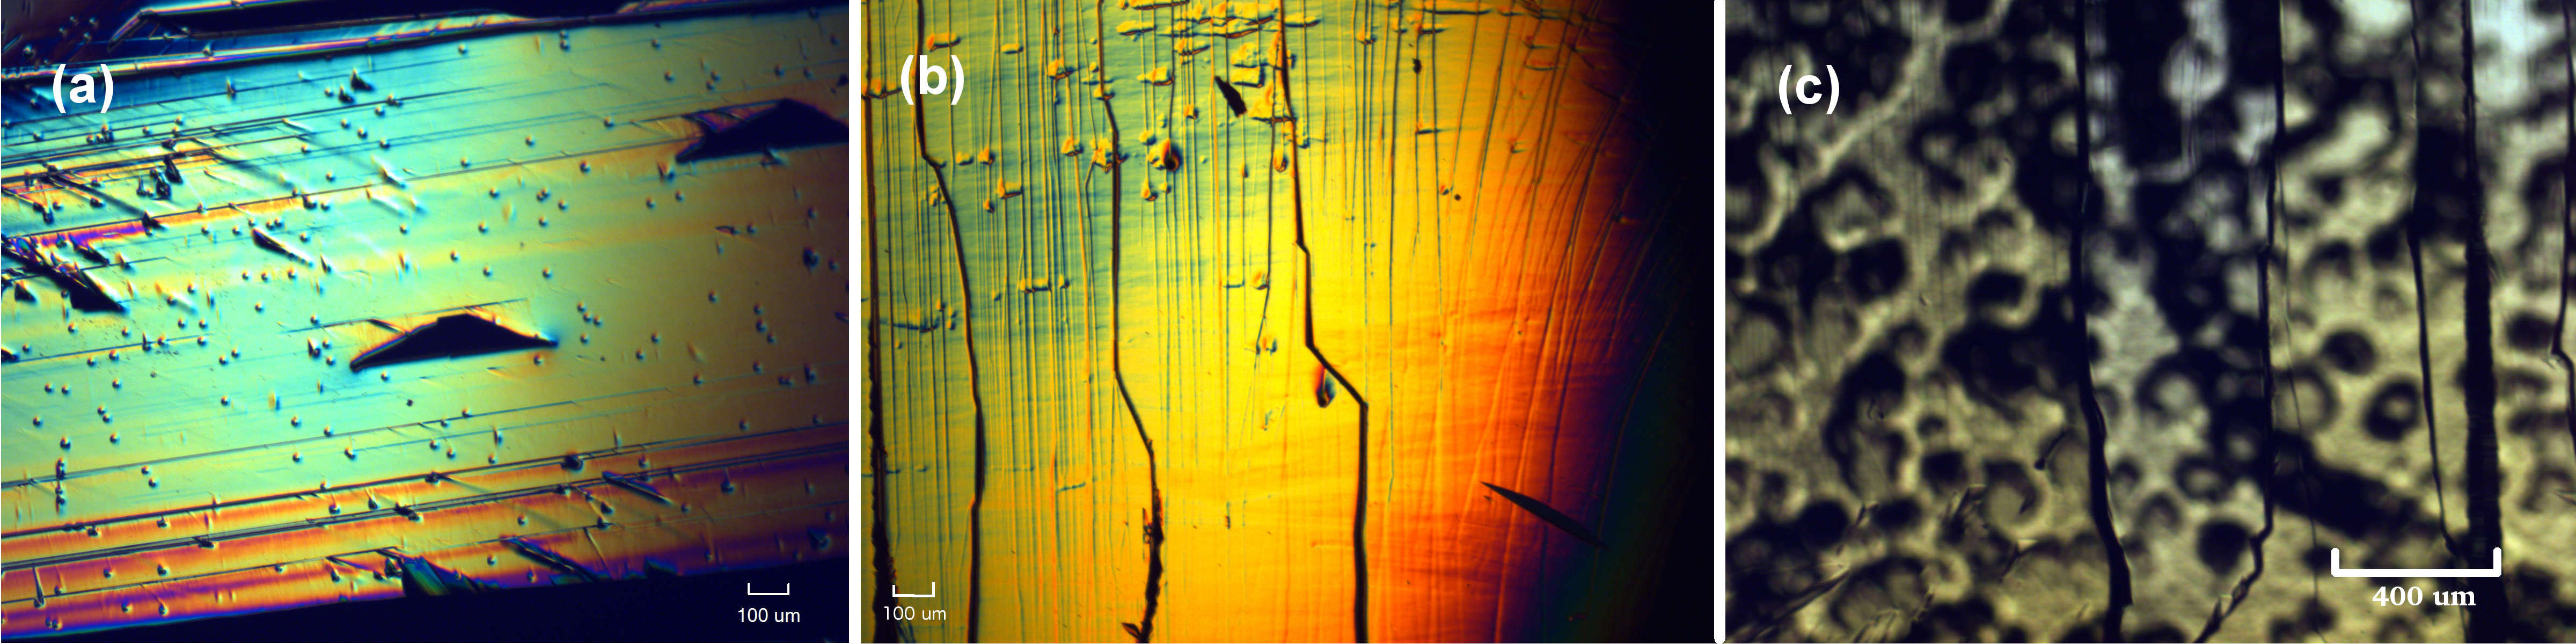
\includegraphics[scale=0.07]{direct_indirect_e20.jpg}
\caption{Reflection micrographs of samples D6 (a) and D9 (b), and transmission micrograph of D9 (c). 
\label{fig:BGe20_micrograph}}
\end{center}
\end{figure}



Absorption measurements were done on directly doped samples with different source doping concentrations, samples D1 and D5. The results of these measurements are shown in figure \ref{fig:abs} (a), together with a reference spectrum from an undoped sample (dotted line). In both samples we see the band edge absorption at around 500 nm. A second feature in the doped sample spectra is the peak at around 700 nm, corresponding to the transition between the boron level and CB. This cannot be seen in the undoped sample. The doped samples show no evidence for a VB to boron transition, which should be seen at around 1800 nm, as described in chapter \ref{sec:doping_in_3C}. Absorption was also measured for doped samples D6 and D7, but neither the band edge nor the boron related peaks were seen in these highly doped samples. The dip and the sharp peak at around 900 nm for sample D5 is attributed to  the equipment. The peak is thought to be an error during background subtraction. 

Figure \ref{fig:abs} (b) shows the result of absorption measurements on samples D1 and D8, together with an undoped sample. It should be noted that D8 is an indirectly doped sample. It can be seen that both the doped sample spectra show the same trend. The graphs increase up to a point near the 700 nm B-CB transition energy, where they level out. This is not visible in the undoped sample. It can further be seen that sample D8 has its B-CB maximum at a slightly shorter wavelength compared to sample D1, which is attributed to the fact that measurements were done on D8 before polishing. The peak shift is in fact a substrate artefact. Absorption measurements were also done on sample D9, which did not show the B-CB peak. 

\begin{figure}[H]
\begin{center}
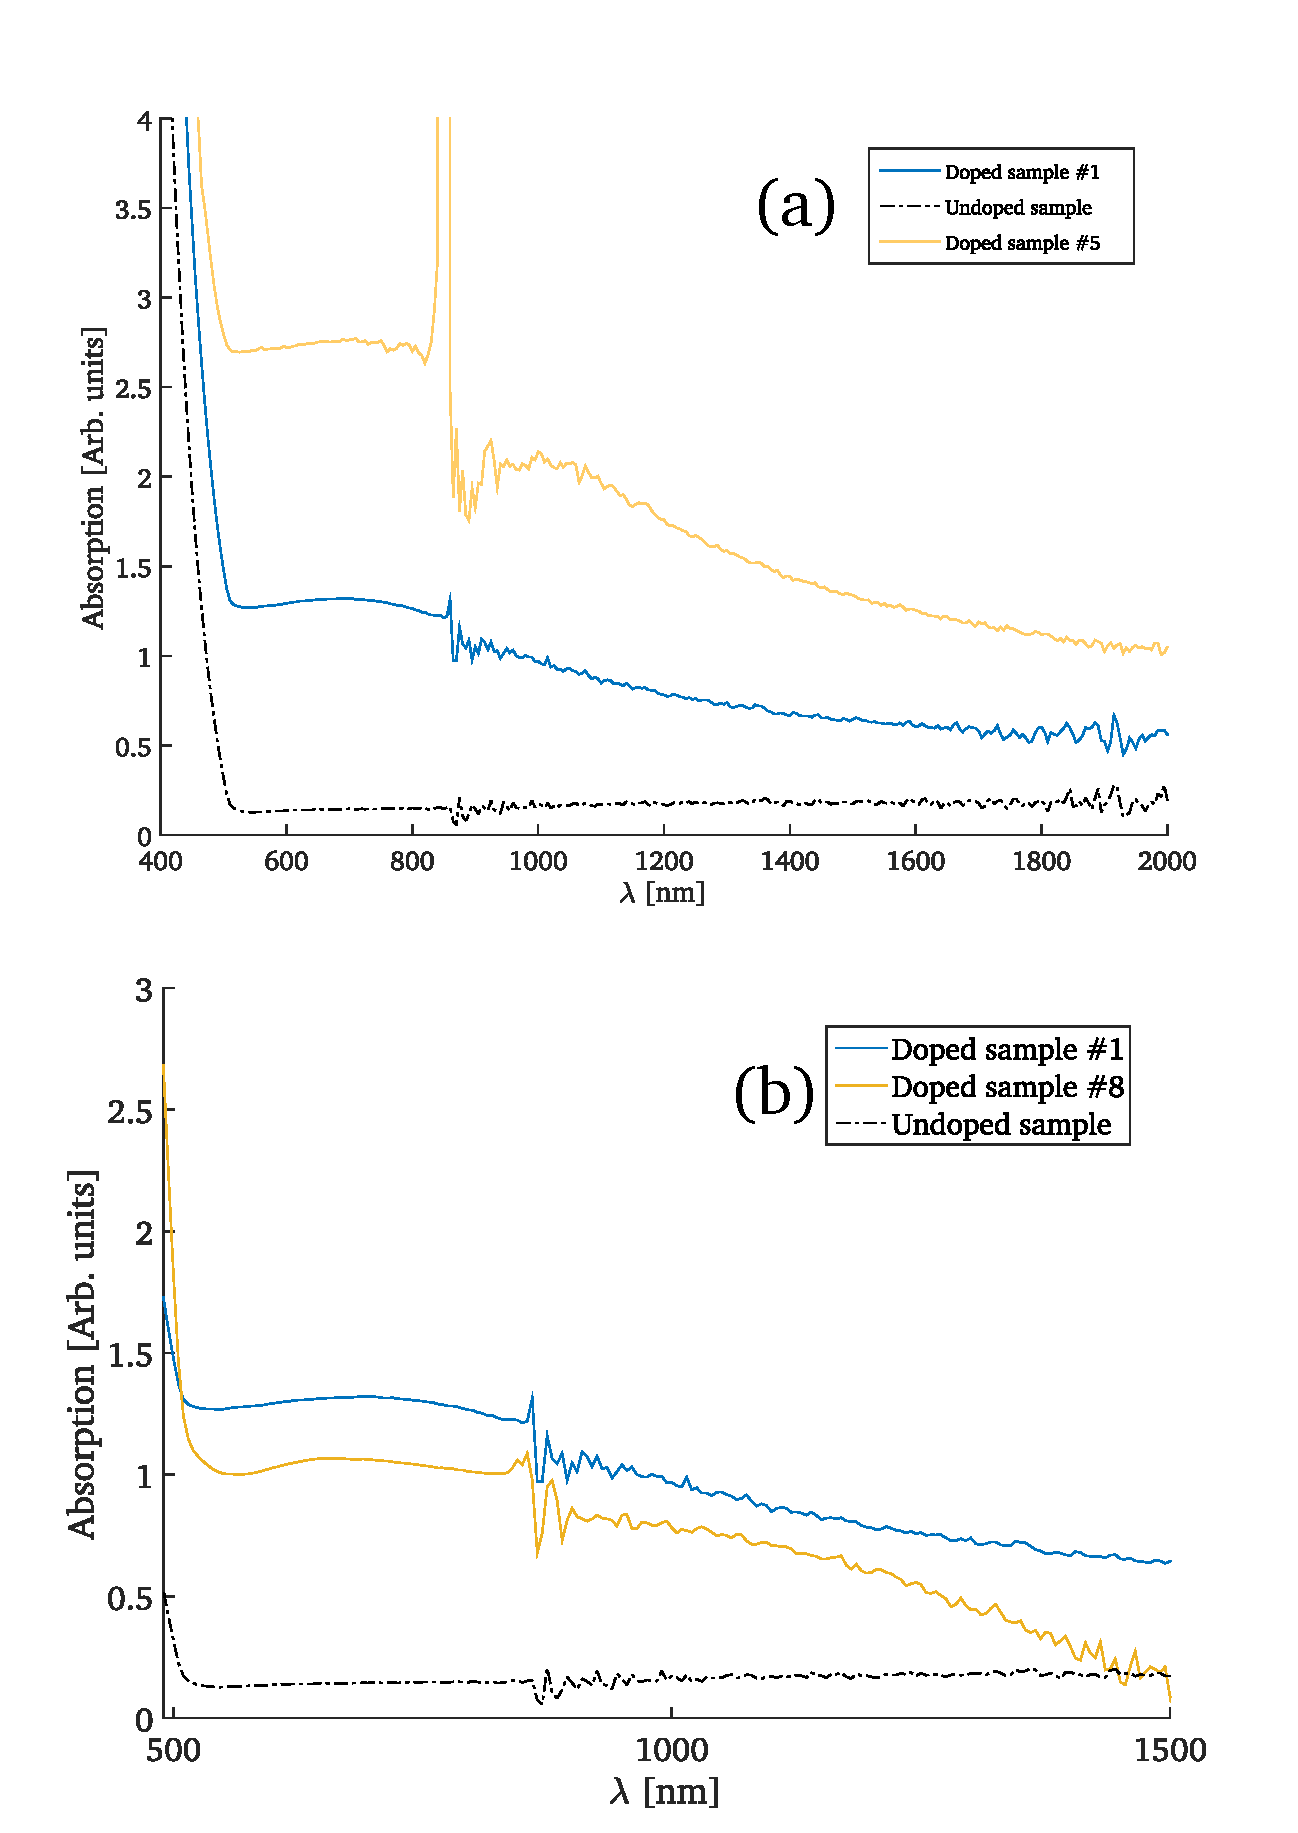
\includegraphics[scale=0.6]{absorption.pdf}
\caption{
(a): Absorption spectrum of undoped sample (dotted line), doped sample D5 (bright yellow line) and doped sample D1 (dark blue line). \\ \\
(b): Absorption spectrum of doped samples D8 (bright yellow line) and D1 (dark blue line), shown together with an undoped sample (dotted line). 
\label{fig:abs}}
\end{center}
\end{figure}

\newpage
LTPL-measurements were done on boron doped samples and on an undoped seed. Figure \ref{fig:pl_spectrum1} shows the resulting spectrum of the undoped seed. Five peaks can clearly be seen in the spectrum, labeled as ZPL and phonon replicas. It should be noted that the ZPL is significantly smaller than the phonon replicas. It can further be seen that several smaller peaks appear on the low energy side of the phonon replicas. These lines originate from exciton complexes.  

\begin{figure}[h]
\begin{center}
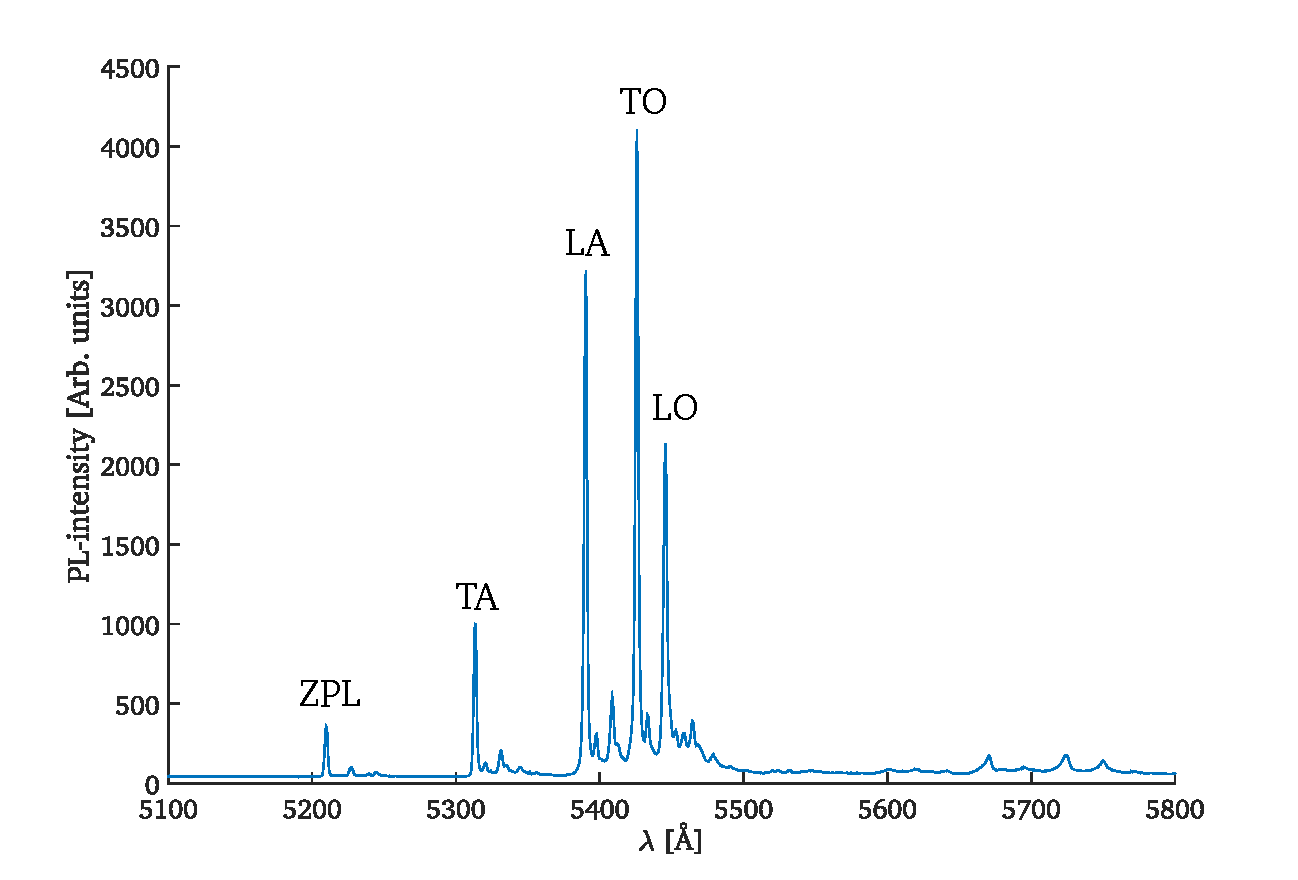
\includegraphics[scale=0.5]{PL_plot1.pdf}
\caption{LTPL spectrum of an undoped seed. The five main peaks are labeled as ZPL and phonon replicas. 
\label{fig:pl_spectrum1}}
\end{center}
\end{figure}

As described in chapter \ref{sec:pl}, the strain in a crystal can be estimated by the fraction between the LA and TO lines. From figure \ref{fig:pl_spectrum1} this is found to be 
\[I_\mathrm{LA}/I_\mathrm{TO} = 0.783.\]
Again as described in the same chapter, the donor concentration can be found from the full width at half maximum (FWHM) of the TA-peak. The FWHM is found to be $\Gamma_{TA} = 1.094$ meV, giving a nitrogen concentration of 
\[[N] \approx 10^{16} \, \mathrm{cm^{-3}}.\]
This value was obtained by using the same parameters as proposed by Camassel et al. \cite{Camassel2006}. 

Doped samples D1, D4 and D6 were measured using LTPL. Not one of these samples show any luminescence, neither from the boron related energy level, nor from the band to band transition. Sample D9 did show some luminescence. It was the only B-doped sample to do so. The sample showed a peak at 5946 Å. At some points it also showed a peak at XXX Å. The spectrum is shown in figure \ref{fig:pl_spectrum2}. 

<Figure>.


































